
\let\negmedspace\undefined
\let\negthickspace\undefined
\documentclass[journal]{IEEEtran}
\usepackage[a5paper, margin=10mm, onecolumn]{geometry}
%\usepackage{lmodern} % Ensure lmodern is loaded for pdflatex
\usepackage{tfrupee} % Include tfrupee package

\setlength{\headheight}{1cm} % Set the height of the header box
\setlength{\headsep}{0mm}     % Set the distance between the header box and the top of the text

\usepackage{gvv-book}
\usepackage{gvv}
\usepackage{cite}
\usepackage{amsmath,amssymb,amsfonts,amsthm}
\usepackage{algorithmic}
\usepackage{graphicx}
\usepackage{textcomp}
\usepackage{xcolor}
\usepackage{txfonts}
\usepackage{listings}
\usepackage{enumitem}
\usepackage{mathtools}
\usepackage{gensymb}
\usepackage{comment}
\usepackage[breaklinks=true]{hyperref}
\usepackage{tkz-euclide} 
\usepackage{listings}
\def\inputGnumericTable{}                                 
\usepackage[latin1]{inputenc}                                
\usepackage{color}                                            
\usepackage{array}                                            
\usepackage{longtable}                                       
\usepackage{calc}                                             
\usepackage{multirow}                                         
\usepackage{hhline}                                           
\usepackage{ifthen}                                           
\usepackage{lscape}
\begin{document}

\bibliographystyle{IEEEtran}
\vspace{3cm}

\title{3.3.3}
\author{AI25BTECH11019 - MENAVATH SAI SANJANA}
% \maketitle
% \newpage
% \bigskip
{\let\newpage\relax\maketitle}

\renewcommand{\thefigure}{\theenumi}
\renewcommand{\thetable}{\theenumi}
\setlength{\intextsep}{10pt} % Space between text and floats

\numberwithin{equation}{enumi}
\numberwithin{figure}{enumi}
\renewcommand{\thetable}{\theenumi}

\textbf{Question}:\\
Construct an equilateral triangle $\triangle ABC$ with each side $5\,\text{cm}$.
\\
\bigskip
\textbf{Solution: }

\begin{align}
\vec{A} &= \myvec{0\\0}, \quad 
\vec{B} = \myvec{5\\0}, \quad 
\vec{C} = \myvec{x\\y}.
\end{align}

Using the cosine rule for $\triangle ABC$:
\begin{align}
BC^2 &= AB^2 + AC^2 - 2(AB)(AC)\cos \angle A 
\end{align}

Since $AB=AC=BC=5$:
\begin{align}
25 &= 25 + 25 - 2\cdot25\cos \angle A 
\end{align}

From (0.3):
\begin{align}
\cos \angle A &= \frac{1}{2}, \quad \angle A = 60^\circ 
\end{align}

Coordinates of $C$:
\begin{align}
\vec{C} &= \myvec{5\cos60^\circ\\5\sin60^\circ}
= \myvec{\tfrac{5}{2}\\\tfrac{5\sqrt{3}}{2}}
\end{align}

\vspace{1cm}

\noindent\textbf{Conclusion:}  
The equilateral triangle $\triangle ABC$ with side $5\,\text{cm}$  
has vertices
\begin{align}
\vec{A}=\myvec{0\\0},\quad 
\vec{B}=\myvec{5\\0},\quad 
\vec{C}=\myvec{\tfrac{5}{2}\\\tfrac{5\sqrt{3}}{2}}.
\end{align}

\begin{figure}[ht!]
    \centering
    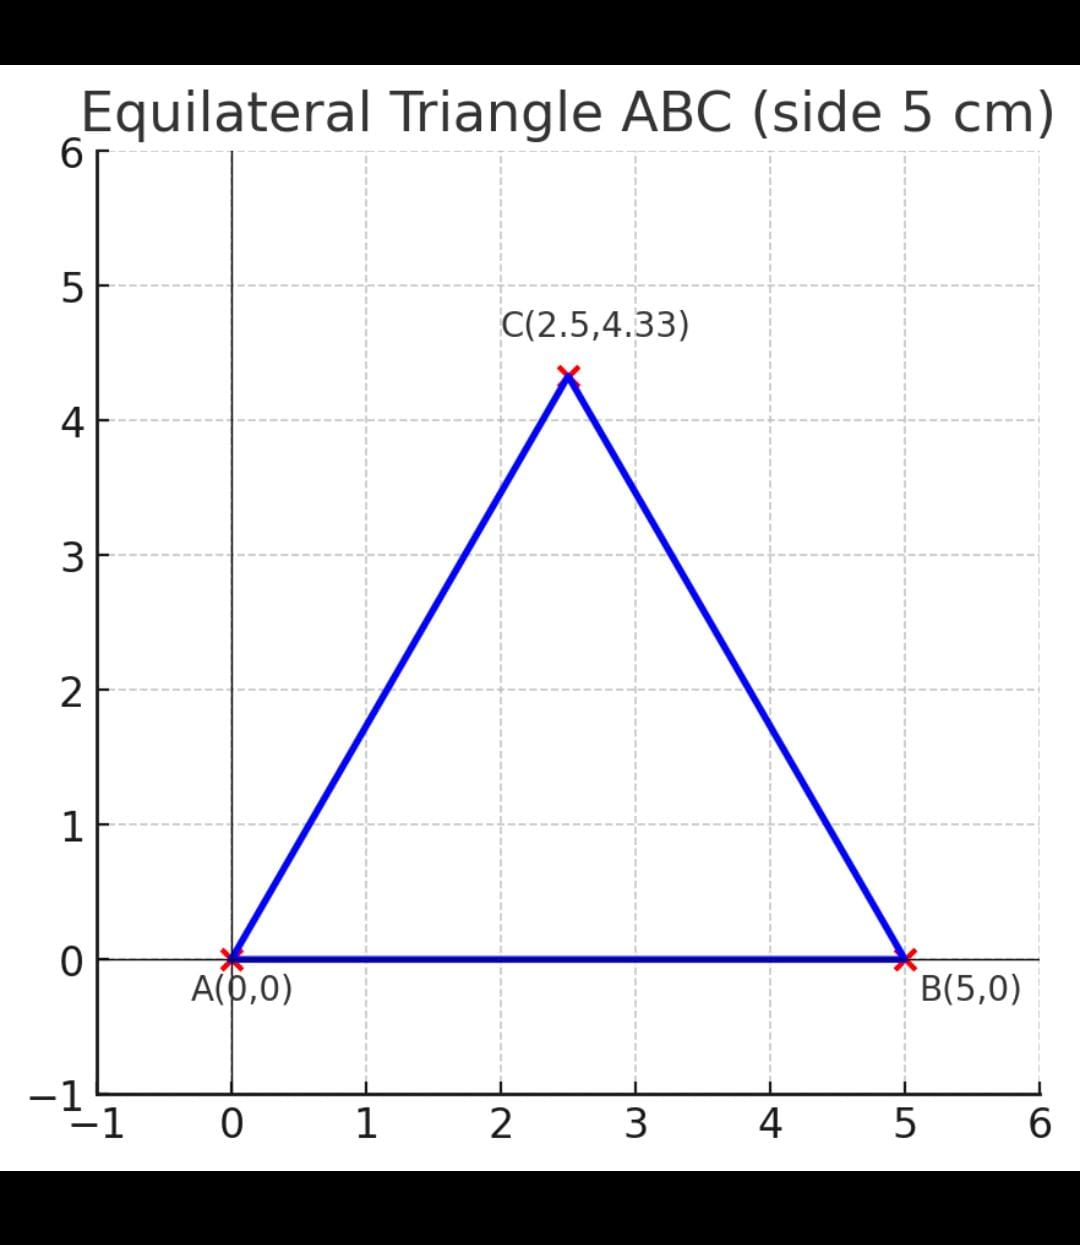
\includegraphics[width=0.8\textwidth]{figs/matgeo-3.3.3.jpeg}
    \caption{}
    \label{fig:1.2.28.jpg}
\end{figure}

\end{document}
